\documentclass{lzureport}

\usepackage{caption}
\usepackage[dvipsnames]{xcolor}  % 更全的色系
\usepackage{listings}  % 排代码用的宏包

\usepackage{booktabs}
\usepackage{float}
\usepackage{tabularx,array,makecell}
%\usepackage{color,xcolor}
%\usepackage{cases}
%\usepackage{mathtools}
%\usepackage{tcolorbox}
%\usepackage{tikz}

%%%%%%%%%%%%%%%%%%%%%%%%%%%%%%%%%%%%%%%%
%% listings设置
%%%%%%%%%%%%%%%%%%%%%%%%%%%%%%%%%%%%%%%%
\lstset{
	language = Python,
	backgroundcolor = \color{yellow!10},    % 背景色:淡黄
	basicstyle = \small\ttfamily,           % 基本样式 + 小号字体
	rulesepcolor= \color{gray},             % 代码块边框颜色
	breaklines = true,                  % 代码过长则换行
	numbers = left,                     % 行号在左侧显示
	numberstyle = \small,               % 行号字体
	keywordstyle = \color{blue},            % 关键字颜色
	commentstyle =\color{green!100},        % 注释颜色
	stringstyle = \color{red!100},          % 字符串颜色
	frame = shadowbox,                  % 用(带影子效果)方框框住代码块
	showspaces = false,                 % 不显示空格
	columns = fixed,                    % 字间距固定
	%escapeinside={<@}{@>}              % 特殊自定分隔符:<@可以自己加颜色@>
	morekeywords = {as},                % 自加新的关键字(必须前后都是空格)
	deletendkeywords = {compile}        % 删除内定关键字;删除错误标记的关键字用deletekeywords删!
}

\major{统计学}
\name{陈祥蔚}
\title{数据结构与卷积神经网络代码实现}
\stuid{320190930061}
\college{数学与统计学院}
\date{\zhtoday}
\expname{数据结构大作业}
\course{数据结构与卷积神经网络代码实现}


\begin{document}

\makecover

\begin{abstract}
	本次大作业主要完成了以下内容:编写两个数据结构、将待学习数据加载到数据结构中、通过神经网络学习、以及比较不同的数据结构的性能。
	
	我选择的两个数据结构是线性表和链表。我编写了这两个数据结构,并且添加了不同的成员变量和成员函数,用来实现不同的功能。
	
	由于无论是什么数据结构,其提供给神经网络用于学习的数据是一样的,而神经网络的训练轮次多,训练量大,因此我选择在训练前的数据处理部分比较不同的数据结构的优劣。评价大致分为三个任务上时间和空间共六个指标,每个指标均进行了12次实验,最后绘图比较。
	
	第一个任务为将图片信息加载到数据结构中。在这个任务中,链表在时间和空间上都不占优,链表所花时间的均值为0.002141秒,所占用内存均值为0.3197MB, 线性表所花平均时间为0.00052秒,所占用内存均值为0.0915MB,链表所花时间为线性表的4倍左右,所占用内存是线性表的3倍左右。
	
	第二个任务为将训练数据和训练标签匹配。在这个任务中,链表在时间上表现优于线性表,所花时间均值为20.782秒,而线性表所花时间为23.4787秒,链表比线性表快了12.98\%左右,但是这一优势可以看出是牺牲了空间所带来的,因为链表的占用内存均值为115.4333MB,而线性表占用内存均值为114.7891MB,不过这一差距并不明显,线性表只比链表少了0.056\%左右,因此可以设想,如果针对更加大量的数据,链表在时间上的优势完全可以弥补空间上的劣势。
	
	第三个任务为将数据转换为神经网络能够接受的类型。在这个任务中,链表依然都不占优,其花费时间的均值为0.000583,占用内存的均值为0.124MB,而线性表的所花时间均值为0.000124,占用内存均值为0.0169MB,链表花费时间约为线性表的5倍,占用的空间为线性表的7倍左右。
	
    在神经网络中,我使用了5个卷积层,前4个卷积层每个后面跟随了一个最大池化层,第2、4、5个卷积层后增加了随机失活层,最后添加了2层全连接层。除了最后一层因为是分类任务所以使用了Softmax层外,其余均使用的是ReLU激活函数。在训练过程中,采用了SGD优化器,开始设置了100个训练轮次,而后经过测试发现在175个训练轮次后训练准确率趋于稳定,测试准确率在72.5\%上下。
    
\end{abstract}

\textbf{关键词:} 深度学习,人工智能
\newpage

\thispagestyle{empty}
\tableofcontents
\newpage 
\setcounter{page}{1}


\section{任务描述}
\noindent 本次作业旨在实现以下目标:

\noindent 1、选择两种数据结构,表示肺部X射线图像和相关的疾病标签

\noindent 2、使用MindSpore构建CNN模型,进行图像分类和疾病检测任务

\noindent 3、将肺部X射线图像加载到数据结构中,包括每个图像的标签,表示是否有特定的疾病。

\noindent 4、训练模型,以自动检测疾病病灶的位置和类型

\noindent 5、评估模型的性能

\noindent 6、分析和比较不同数据结构对于模型性能和数据处理效率的影响

\section{数据结构}
针对图像文件在管理系统中的特性,以及考虑到图像在卷积神经网络中的加载方式,我们采取的管理并储存图像的方式是线性表和链表。

\subsection{线性表}
在线性表中,我们储存的是每个图片在计算机中的地址,由地址对于具体的图片进行管理。在使用CNN网络进行学习的时候,通过传入地址读取具体的图片,并且对于图片进行学习。因此,我们实现了以下的特殊方法:初始化、迭代、求长度;以及以下的自定义方法:返回匹配项下标、添加元素、删除元素、插入元素、查找元素。\\

\noindent LinearTable 类:表示线性表,包含以下主要功能:

\noindent \_\_init\_\_(self):初始化一个空的线性表,使用列表 datalist 存储数据。

\noindent \_\_iter\_\_(self):使线性表可迭代,可以直接迭代线性表中的元素。

\noindent \_\_len\_\_(self):返回线性表中元素的数量。

\noindent index(self, data):返回第一个匹配项的下标,如果不存在则返回 -1。

\noindent add\_data(self, data):向线性表末尾添加一个新的数据项。

\noindent find\_data(self, data):查找线性表中所有匹配指定数据项的下标,返回一个列表。

\noindent insert\_data(self, location, data):在指定位置插入新的数据项。

\noindent delete\_data(self, data):从线性表中删除第一个匹配指定数据项的元素。

\subsection{双向链表}
在LinkedList.py中,我们实现了一个基本的双向链表结构,用于管理图像文件的路径。以下是每个类的主要功能:\\

\noindent ImageNode 类:表示链表中的节点,每个节点包含一个图像文件的路径。节点还包括指向下一个节点和上一个节点的指针。

\noindent ImageLinkedList 类:表示双向链表,包含以下主要功能:

\noindent add\_image(image\_path):向链表末尾添加一个新的图像节点。

\noindent delete\_image(image\_path):从链表中删除包含指定图像路径的节点。

\noindent search(image\_path):在链表中查找包含指定图像路径的节点,返回该节点。

\noindent is\_empty():检查链表是否为空。

\noindent length():返回链表中节点的数量。

\noindent display\_images():打印链表中所有图像节点的路径。

\noindent \_\_getitem\_\_(index):通过索引获取链表中特定位置的图像路径。

\noindent to\_list():将链表中的元素输入到列表中并返回

\subsection{数据加载与测量}
与数据结构和数据加载相关的文件是dshwwithpytorch文件夹中的datawithlt.py和datawithll.py文件,前者是使用线性表,后者是使用链表。\\

在这两个文件中,对数据进行了加载和预处理,并在这个过程中调用了例如time()对于加载时间进行测量,以及导入psutil包对于内存进行测量。直接运行这两个文件夹即可得到初步的结果如下。

\begin{figure}[H]
	\centering
	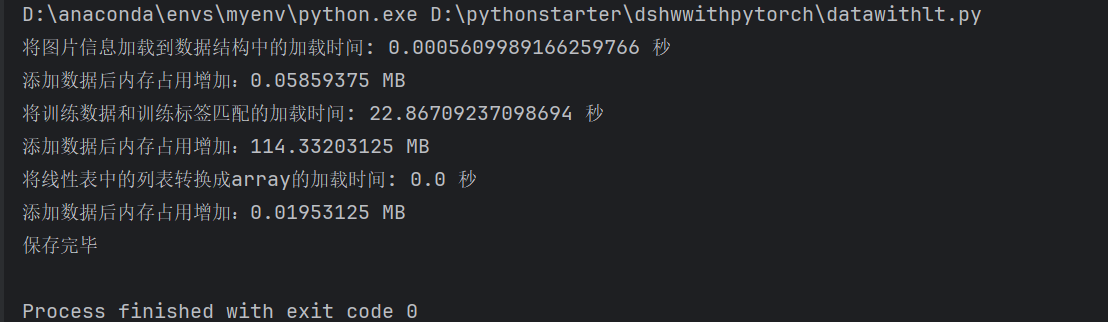
\includegraphics[width=0.8\textwidth]{lt.png}  % 替换为你的图片文件名
	\caption{线性表的运行时间和占用内存}
	\label{fig:example}
\end{figure}

\begin{figure}[H]
	\centering
	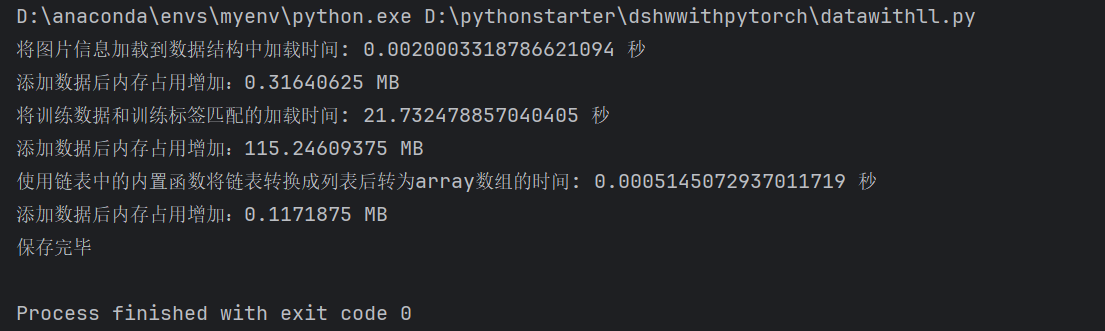
\includegraphics[width=0.8\textwidth]{ll.png}  % 替换为你的图片文件名
	\caption{链表的运行时间和占用内存}
	\label{fig:example}
\end{figure}

\subsection{定量分析}
\subsubsection{方法和评价标准}
在实验中,为了定量分析,准确起见,我将每个数据结构加载了十二次,比较不同的数据结构在不同的指标上的差别,并分析出现这样的结果的原因。与之相关的文件是dshwwithpytorch文件夹里面的comparell.py,comparelt.py,myplot.py,time\&memory文件夹和plots文件夹。在comparell.py,comparelt.py两个文件中我分别用两种数据结构运行了12次,获得实验数据。而后我将数据以列表的形式储存到time\&memory文件夹中。\\

最后,我在myplot.py文件中绘制了比较的图像,而后将图像导出保存至plots文件夹中。分析的指标分为三个进程,共有六个,三个为时间指标,三个为内存指标。它们是:(1)将图片信息加载到数据结构中的加载时间和添加数据后内存占用。(2)将训练数据和训练标签匹配的加载时间和内存占用。(3)将各个数据结构中的数据转换成array数组的加载时间和内存占用。在实验时选取的数据集是训练集。

选择这三项进程的六个指标原因如下。\\

首先,由于创建数据结构的目的就是储存、管理数据,因此选择将图片信息加载到数据结构中的加载时间和添加数据后内存占用是非常自然的事情。\\

其次,由于分类问题需要将数据和标签匹配,因此数据结构在匹配的速度和占用内存大小的性能就成为了评价数据结构的重要指标。\\

最后,不管什么数据结构,由于神经网络只能接受特定的数据类型,因此我们都需要将数据结构中的数据转换数据类型后才能进行学习,因此我们选择了将数据结构中的数据转换成array数组的加载时间和内存占用作为两个评价指标。
\subsubsection{将图片信息加载到数据结构中的加载时间和内存占用}
\begin{figure}[H]
	\centering
	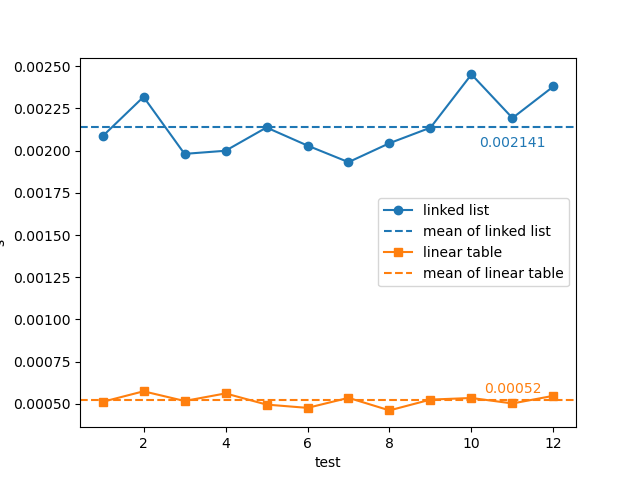
\includegraphics[width=0.7\textwidth]{time1}  % 用于插入图片的命令
	\caption{将图片信息加载到数据结构中的加载时间}
	\label{fig:your_label}
\end{figure}
\begin{figure}[H]
	\centering
	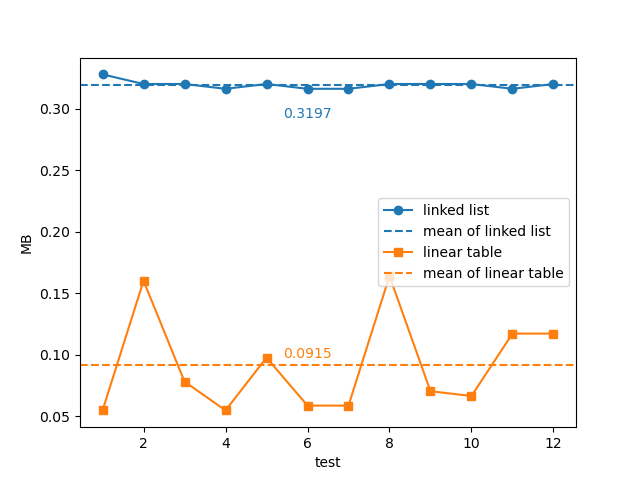
\includegraphics[width=0.7\textwidth]{memory1}  % 用于插入图片的命令
	\caption{将图片信息加载到数据结构中的内存占用}
	\label{fig:your_label}
\end{figure}
根据图表可以看出,从时间上来看,链表花费的时间是线性表的4倍左右,链表占用的内存是线性表的3倍左右。据分析,这样的结果产生的原因是在加载阶段,链表的每一个节点要比线性表多创建了头指针和尾指针,因此不管是加载时间还是占用内存,链表都比线性表要花更多的时间。
\subsubsection{将训练数据和训练标签匹配的加载时间和内存占用}
\begin{figure}[H]
	\centering
	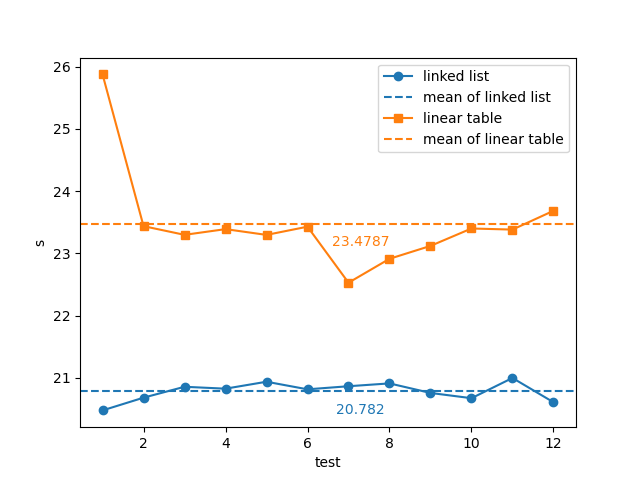
\includegraphics[width=0.7\textwidth]{time2}  % 用于插入图片的命令
	\caption{将训练数据和训练标签匹配的加载时间}
	\label{fig:your_label}
\end{figure}
\begin{figure}[H]
	\centering
	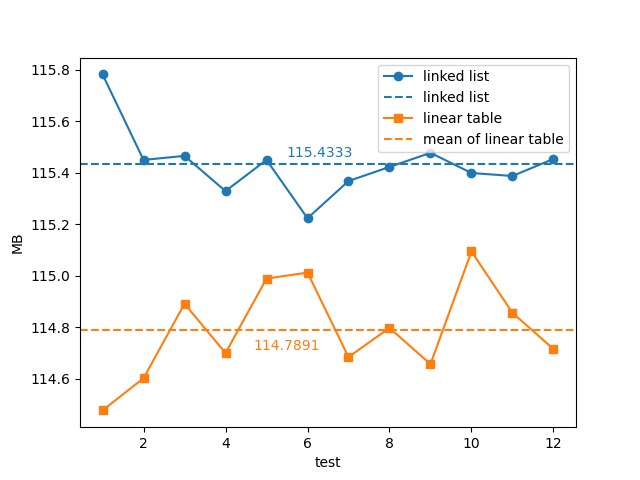
\includegraphics[width=0.7\textwidth]{memory2}  % 用于插入图片的命令
	\caption{将图片信息加载到数据结构中的内存占用}
	\label{fig:your_label}
\end{figure}
在这两个指标中,链表的加载时间普遍低于线性表,内存占用普遍高于线性表,但是差别并不明显。原因可能链表可以动态开辟存储空间,因此在匹配的过程中时间较短,但是由于每个节点都有指针,因此总体内存增大。
\subsubsection{将各个数据结构中的数据转换成array数组的加载时间和内存占用}
\begin{figure}[H]
	\centering
	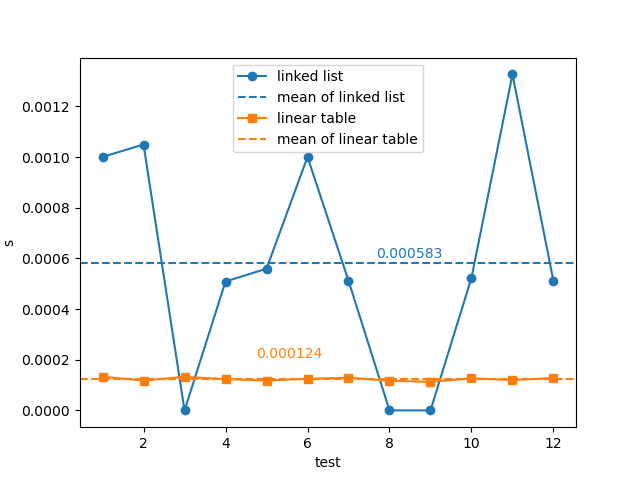
\includegraphics[width=0.7\textwidth]{time3}  % 用于插入图片的命令
	\caption{将各个数据结构中的数据转换成array数组的加载时间}
	\label{fig:your_label}
\end{figure}
\begin{figure}[H]
	\centering
	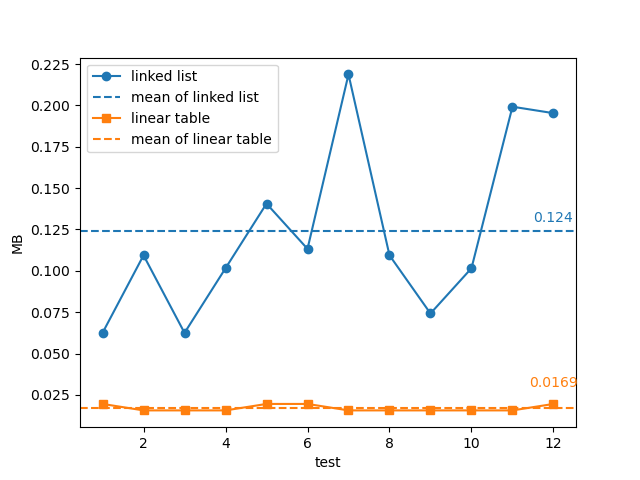
\includegraphics[width=0.7\textwidth]{memory3}  % 用于插入图片的命令
	\caption{将图片信息加载到数据结构中的内存占用}
	\label{fig:your_label}
\end{figure}
在转换数组的这两个指标中,链表的加载时间是线性表的6倍左右,占用内存是线性表的7倍。原因应当如下:线性表在储存信息的时候就是采取的列表形式,因此按照线性表的顺序逐一转换即可;而链表由于分散储存,因此需要在链表中写一个转换成线性表的函数,才能将链表中的元素先储存进一个列表中,而后才能进一步转换为数组。

\subsection{误差}
首先在实验的时候犯了一个错误,如图是将训练数据和训练标签匹配的加载时间的图像。从图中可以看出,第一次实验后内存便基本为零了。猜想的原因是,线性表的实验过程中是用for循环进行实验的,但是可能在这个过程中需要清空内存,但是没有清空,于是就出现了这样的情况。
\begin{figure}[H]
	\centering
	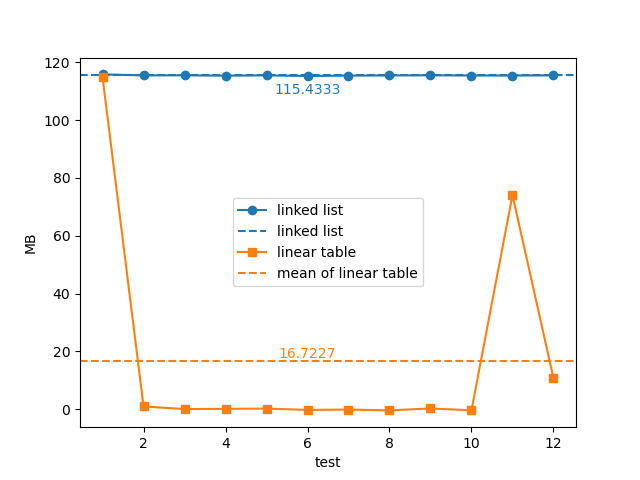
\includegraphics[width=0.7\textwidth]{wrong1}  % 用于插入图片的命令
	\caption{错误图样}
	\label{fig:your_label}
\end{figure}
因此保险起见,我后来分别将线性表和链表的单次实验进行了12次,并手动将数据储存进线性表中。原始数据可以在comparell.py和comparelt.py中看到,也就是上面几节中图片展示的样子。但是明显可以看出,有的数据波动过大,例如2.4.4节中的图7,图8,目前并不是很清楚原因是什么。\\

另外,在实验过程中偶尔会出现时间或内存为0.0的状况,时间为0.0的原因应该是使用了time包中的time()函数进行计时,后来换成perf\_counter()函数后就不会出现这样的状况了。






\section{数据集}
数据集来源于https://www.kaggle.com/datasets/paultimothymooney/chest-xray-pneumonia/code?datasetId=17810\&sortBy=voteCount,该数据集分为 3 个文件夹(train、test、val),并包含每个图像类别(肺炎/正常)的子文件夹。有 5,863 张 X 射线图像 (JPEG) 和 2 个类别(肺炎/正常)。

胸部 X 射线图像(前后位)选自广州市妇女儿童医疗中心 1 至 5 岁儿童患者的回顾性队列。所有胸部 X 射线成像均作为患者常规临床护理的一部分进行。

为了分析胸部 X 射线图像,首先通过删除所有低质量或不可读的扫描来筛选所有胸部 X 射线照片以进行质量控制。然后,两位专家医生对图像的诊断进行了分级,然后才允许训练人工智能系统。为了解决任何评分错误,评估集还由第三位专家进行了检查。

\section{预处理}
为了能够进行CNN的训练,我们需要对于现有的数据进行一些预处理。预处理的文件是mydata.py,处理后的数据存放在data文件夹中,该文件夹中包括了test\_data.npy,test\_data.npy,train\_label.npy,train\_data.npy,val\_data.npy,val\_label.npy。

预处理包括了以下步骤:

\noindent1、定义获取图片路径的函数: get\_photo\_paths 函数接受一个文件夹路径作为参数,检查该文件夹是否存在,获取文件夹中的所有文件,并返回包含这些文件路径的列表。

\noindent2、定义加载训练数据的函数: get\_training\_data 函数接受两个线性表对象作为参数,用于存储数据和对应的标签。函数根据文件路径加载图像数据,将其调整大小,然后添加到数据线性表中,并根据文件路径中是否包含特定标签确定对应的标签。

\noindent3、初始化线性表和获取图片路径列表: 创建三个线性表对象 train、test、val,并通过 get\_photo\_paths 函数获取训练、测试和验证集的图像文件路径。

\noindent4、将图片信息加载到线性表中: 使用 add\_data 方法将图像信息加载到训练、测试和验证集的线性表中。

\noindent5、建立用于存放标签的线性表: 创建三个线性表对象 train\_data\_label、test\_data\_label、val\_data\_label,用于存放对应的标签信息。

\noindent6、获取训练数据: 调用 get\_training\_data 函数获取训练、测试和验证集的图像数据,并将其归一化。

\noindent7、预处理: 将图像数据的形状修改为在代码中定义的 img\_size(150)。

\noindent8、转换数据类型: 将图像数据和标签的数据类型转换为适用于 MindSpore 框架的数据类型。

\noindent9、修改标签的形状: 使用 np.squeeze 函数将标签的形状进行修改。

\noindent10、保存文件: 将处理后的图像数据和标签保存为 .npy 文件,以备后续在 MindSpore 中使用。
\section{CNN}
\noindent 1、卷积层(Convolutional Layers):

使用了五个卷积层,每一层包括卷积操作(nn.Conv2d)、批量归一化(nn.Batch\\Norm2d)、激活函数(ReLU)和最大池化(nn.MaxPool2d)。
卷积核大小为 (3, 3),步长(stride)为 1,padding 模式为 'same',保证了卷积后特征图大小不变。

\noindent 2、Dropout 层:

在第二、四、五个卷积层后使用了 Dropout 操作,有助于防止过拟合。

\noindent 3、全连接层(Fully Connected Layers):

包括两个全连接层,每一层包括全连接操作(nn.Dense)、激活函数(ReLU)和 Dropout 操作。
第一个全连接层的输出大小为 128,输入大小为 6400(由 nn.Flatten 层展平得到)。
第二个全连接层的输出大小为 3,对应于分类的类别数量。

\noindent 4、激活函数:

使用了 ReLU 激活函数,除了最后一层,最后一层使用了 Softmax 激活函数进行多类别分类。
打印操作:

在网络中使用了 P.Print() 操作,该操作用于在计算过程中打印张量的形状信息。
网络的整体结构是卷积层的堆叠,通过不断降低特征图的大小,最终通过全连接层输出分类结果。 Dropout 层有助于提高模型的泛化能力。
\begin{figure}[H]
	\centering
	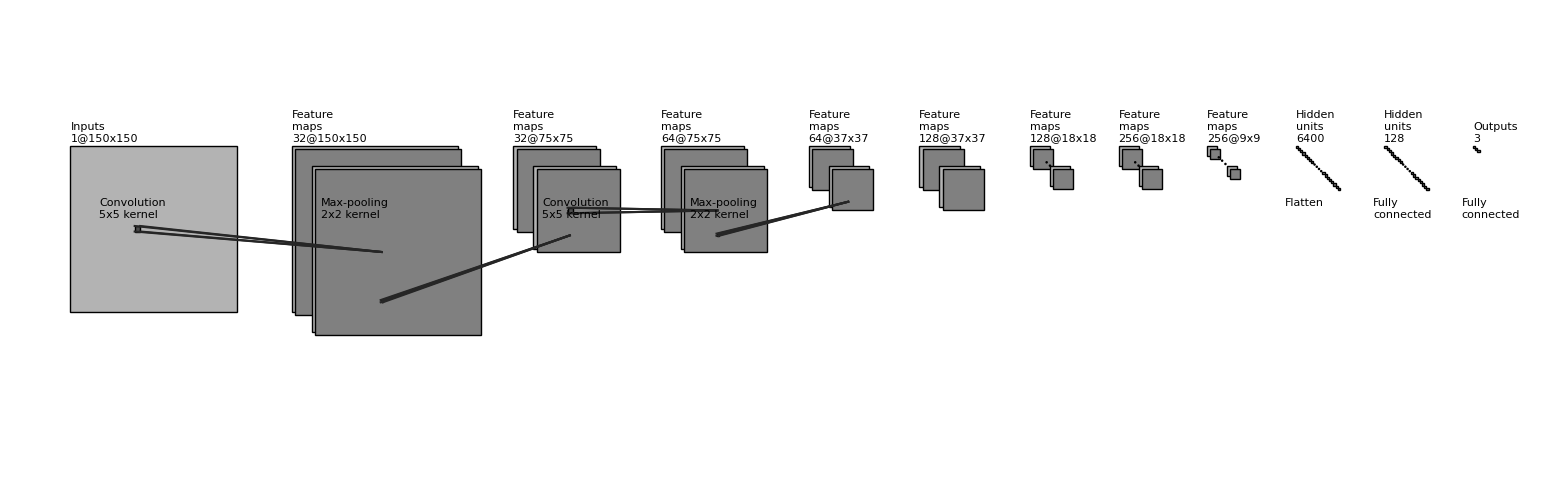
\includegraphics[width=1\textwidth]{convnet_fig.png}
	\caption{CNN网络图像}
	\label{fig:example}
\end{figure}

\section{训练}
\noindent 1、优化器和损失函数的设置: 使用随机梯度下降 (SGD) 作为优化器,学习率为 0.01。
使用交叉熵损失函数 (CrossEntropyLoss)。\\
\noindent 2、训练循环:设置了总共 100 个训练周期 (epochs)。
在每个周期内,遍历训练数据集,并进行前向传播、反向传播和优化。
输出每个步骤的训练进度信息,包括当前周期和步骤。\\
\noindent 3、模型保存:在训练完成后,将模型保存到文件 'model/model.pth'。\\
\noindent 4、损失和准确率的记录:记录每个训练周期的总损失和准确率。
绘制训练损失和准确率随着训练周期变化的图表。\\
\noindent 5、100个轮次训练结果为:总损失803.9553998112679,准确率0.9351993865030674
\noindent 图像如下:
\begin{figure}[H]
	\centering
	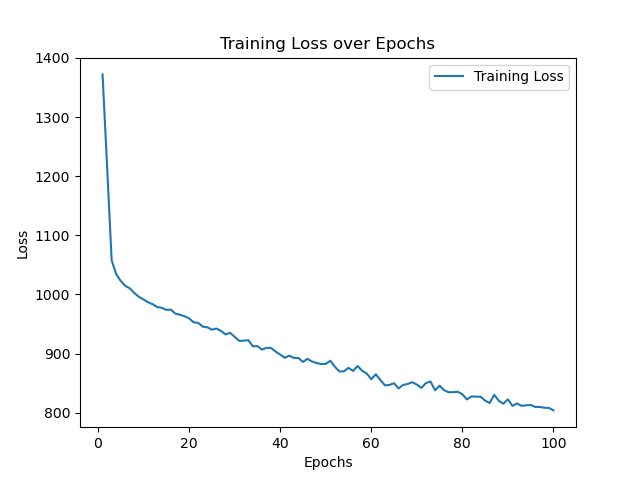
\includegraphics[width=0.7\textwidth]{loss_plot.png}
	\caption{损失值随训练轮次变化}
	\label{fig:example}
\end{figure}

\begin{figure}[H]
	\centering
	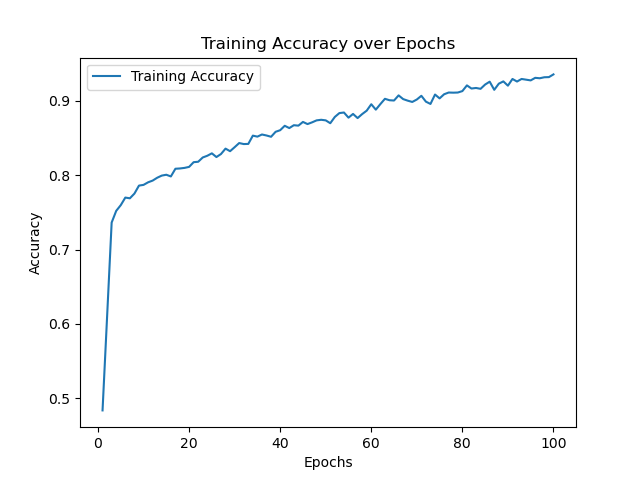
\includegraphics[width=0.7\textwidth]{accuracy_plot.png}
	\caption{准确率随训练轮次变化}
	\label{fig:example}
\end{figure}
\section{测试}
在测试中,我首先比较了在50、100、150、200、250、300轮次中损失值和准确率的变化,可以发现在150-200轮次,损失值和准确率就开始不再变化。
\begin{figure}[H]
	\centering
	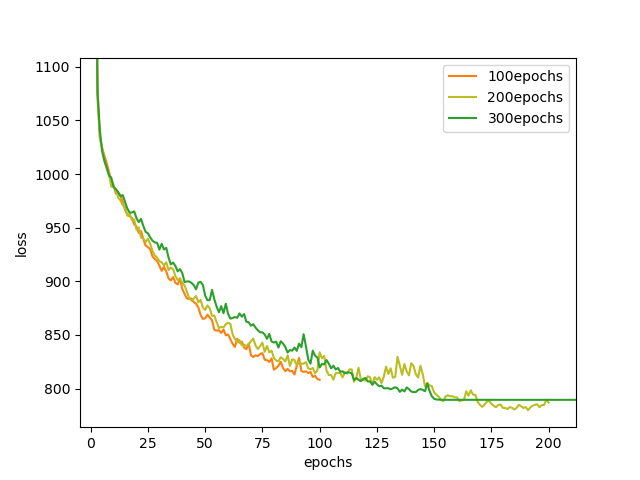
\includegraphics[width=0.7\textwidth]{loss3.png}
	\caption{损失值随训练轮次变化}
	\label{fig:example}
\end{figure}
\begin{figure}[H]
	\centering
	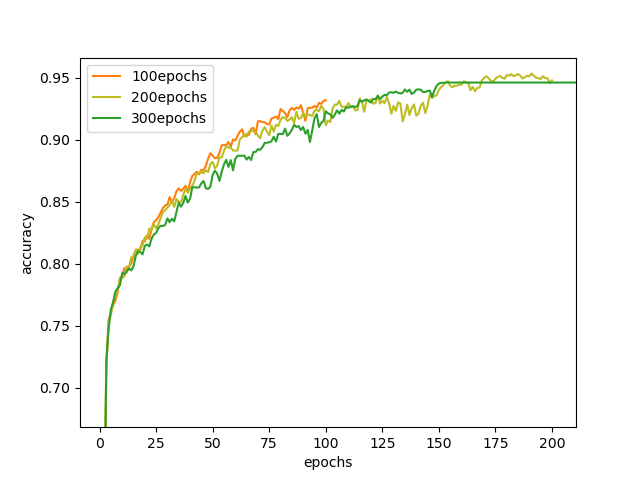
\includegraphics[width=0.7\textwidth]{acc3.png}
	\caption{准确率随训练轮次变化}
	\label{fig:example}
\end{figure}

\newpage
因此,我们将准确率的测试放在175次进行。结果如图所示。
\begin{figure}[H]
	\centering
	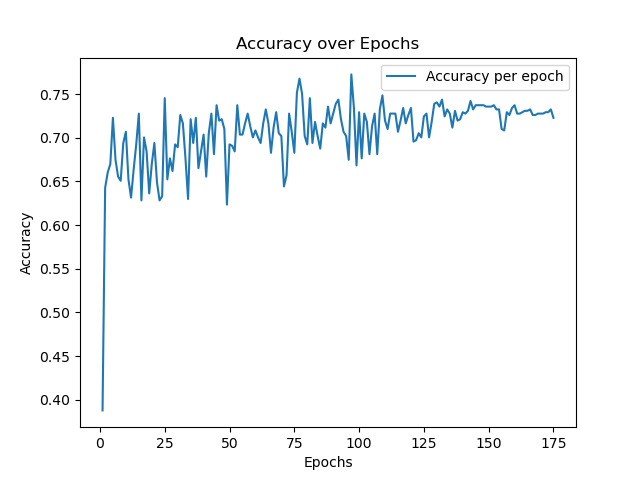
\includegraphics[width=0.7\textwidth]{accperepoch.png}
	\caption{175轮次准确率随轮次变化}
	\label{fig:example}
\end{figure}
从图片中可以看出,准确率在70\%上下徘徊,并不稳定,最后可能是收敛到72.5\%左右,相对来说并不高。模型还有很大的进步空间。

% \section{结果}
简要描述任务的背景和目标。

\section{讨论}
\noindent 本次作业中仍然存在着各种不足。\\

\noindent 1、在运行mindspore的时候并不能十分完美地运行出来。神经网络的结构没有问题,在训练的时候发现出了一些问题。在训练的时候loss值一直不收敛。后来发现标签不同,loss值收敛到不同的值,并且最终的测试准确率一直在38\%,保持不变。排查原因时,我认为数据集和预处理没有问题,因为用pytorch写的网络是可以运行出来的,并且MindSpore中的训练方法是导入Model包,而后直接调用里面的model\_train函数进行训练,因此不太清楚是哪里出现问题了。另外一个重要的原因是MindSpore在Windows上不支持GPU计算,用CPU计算会很慢。\\

\noindent 2、代码的组织不好。很多时候直接在作业的文件夹下新建py文件来写一个程序,因此一方面看起来比较乱;并且很多时候导入文件或者保存文件选择的是绝对地址,因此可能不便于在别的计算机上测试。不过还好不管是数据集还是程序文件都基本上是直接在D盘中的,因此就算是绝对地址的话导入也比较方便。\\

\noindent 3、实验代码太过冗长,符号不简洁。因为实验中涉及到两种数据结构和多个指标,因此如何合理地组织符号也是一个问题。上一个问题提出的组织架构不好,一方面也是代码太过冗长的原因,有的时候写的时候没有规划好,写完了一个数据结构的相关部分后,发现另外一个不能在同一个文件中运行,因此只好另写一个文件,导致整个文件夹比较繁杂。

\section{总结}
在本次作业中,研究了线性表和链表就加载数据等方面的性能,综合比较了其在时间和空间上在各个任务中的表现优劣:将数据加载到数据结构中时由于链表要额外创建指针,因此从时间和空间上来说均比线性表表现差一些;将数据彼此匹配时,链表在时间上表现比线性表优异,分析应该是用空间换时间的原因,其相应的空间占用得更多一些;针对数据转换任务,链表在时间和空间上都并不如线性表,原因应该是链表一方面储存了指针,一方面比链表要额外经过一个转换成列表的步骤。

最后,我设计了一个神经网络,并且让神经网络学习,而后进行了不同轮次的训练,比较出训练准确度不再增加的轮次后对于准确度进行测试,完成了神经网络的学习,效果有待提升,可能是网络架构的问题,也可能是优化器等各个方面的问题。


%\newpage
\thispagestyle{empty}
\bibliography{books}
\newpage

\appendix

%\section{串行部分全部实验结果}

图或者代码放上来。

\section{并行部分全部实验结果}

图或者代码放上来。

\end{document}